\section{Shadow DOM}\label{shadow-dom}

Durch Kapselung ist es möglich, Details eines Objektes von anderen Teilen des Programms zu verstecken. Das Programm muss nur wissen, wie es auf die benötigten Funktionen zugreift, jedoch nicht, wie das Objekt die Funktionen intern umsetzt. Dieses Konzept ist in allen objektorientierten Programmiersprachen umgesetzt, jedoch nicht in der Webentwicklung. Beispielsweise kann das \ac{CSS} oder JavaScript, das für ein Element geschrieben ist, auch das \ac{CSS} oder JavaScript anderer Elemente beeinflussen. Je größer das Projekt wird, desto unübersichtlicher und komplexer wird es, zu gewährleisten, dass \ac{CSS} oder JavaScript sich nicht ungewollt auf andere Teile der Webseite auswirkt.

Diesem Problem widmet sich das sogenannte Shadow \ac{DOM}, welches ein Sub-\ac{DOM} unterhalb eines Elements darstellt und es ermöglicht, \ac{HTML} und \ac{CSS} in sich zu kapseln und zu verstecken. Als Kontrast zu Bezeichnung ``Shadow \ac{DOM}'' wird das reguläre \ac{DOM} des Hauptdokuments auch oft als ``Light \ac{DOM}'' bezeichnet. Das Shadow \ac{DOM} wird bereits in \ac{HTML}5 standardmäßig eingesetzt, wie beispielsweise im \texttt{\textless{}input\textgreater{}}-Tag. Beim Inspizieren des Elements mit Hilfe der Chrome Developer Tools (siehe Abbildung \ref{fig:itpelem}) wird deutlich, dass das \texttt{\textless{}input\textgreater{}}-Tag ein Shadow \ac{DOM} beinhaltet, welches das eingegebene Passwort kapselt. \cite[S. 109-126]{citeulike:13844975}

\begin{figure}[htbp]
 \centering
 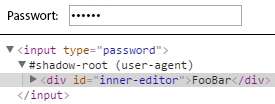
\includegraphics{kapitel2/bilder/3-shadow-dom-input-type-password}
 \caption{Passwort-Input-Element}
 \label{fig:itpelem}
\end{figure}


\subsection{Shadow DOM nach W3C}\label{shadow-dom-nach-w3c}

\begin{figure}[htbp]
 \centering
 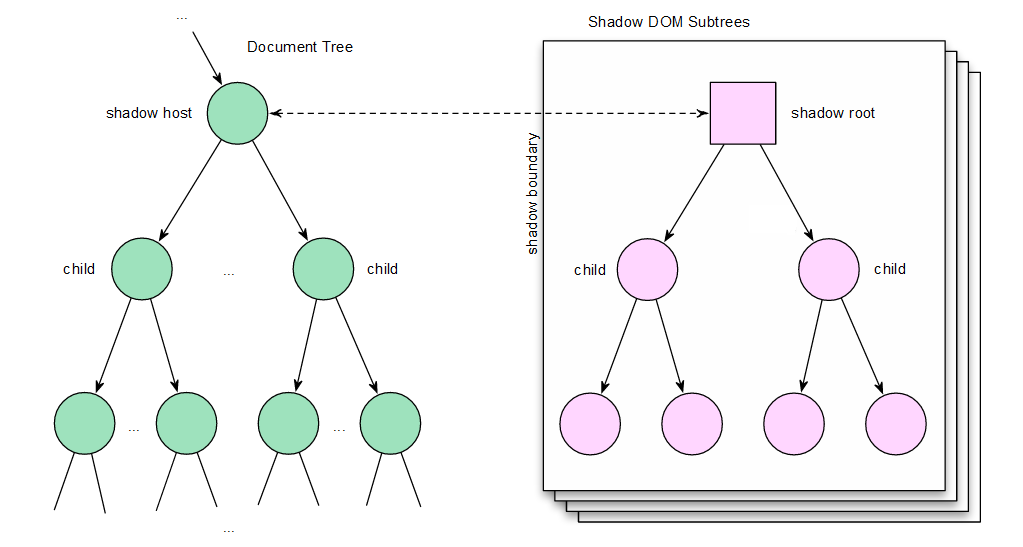
\includegraphics[width=\linewidth]{kapitel2/bilder/3-shadow-dom-shadow-boundary}
 \caption{Shadow \ac{DOM} und Shadow Boundary nach W3C}
 \label{fig:sdsbnw3c}
\end{figure}

Wie auf Abbildung \ref{fig:sdsbnw3c} zu sehen, liegt das Shadow \ac{DOM} dabei parallel zu dem \ac{DOM}-Knoten des beinhaltenden Elements. Ein Knoten im Document Tree (links abgebildet) wird als ``Shadow Host'' - ein Element, welches ein Shadow \ac{DOM} beinhaltet - markiert. Die gestrichelte Linie zeigt die Referenz zu der entsprechenden Shadow \ac{DOM} Wurzel, dem ``Shadow Root''. Die Referenz geht dabei durch die sogenannte ``Shadow Boundary'', welche es ermöglicht, den Shadow \ac{DOM}, und alles was dieser beinhaltet, zu kapseln \cite{citeulike:13851350}. Dies verhindert, dass externes \ac{CSS} oder JavaScript das interne Markup oder umgekehrt internes \ac{CSS} oder JavaScript den Light \ac{DOM} oder andere Shadow \ac{DOM}s ungewollt beeinflussen können. Ein Element kann auch mehrere Shadow \ac{DOM} Wurzeln referenzieren, allerdings wird nur die zuletzt hinzugefügte vom Browser gerendert, da dieser zum Rendern einen \ac{LIFO} Stack benutzt. Dabei wird der zuletzt hinzugefügte Shadow Tree ``Youngest Tree'' genannt, der jeweils zuvor hinzugefügte Shadow Tree wird ``Older Tree'' genannt. Das dynamische Hinzufügen von Shadow \ac{DOM}s ermöglicht es, die Inhalte der Webseite nach dem Rendern zu ändern.


\subsection{Content Projection}\label{content-projection}

Neben dem vom Shadow \ac{DOM} vorgegebenen \ac{HTML}, können auch Inhalte aus dem Light \ac{DOM} in den Shadow \ac{DOM} projiziert werden. Der Shadow \ac{DOM} nimmt dabei die zu projizierenden Inhalte und projiziert sie an der vorgegebenen Stelle im Shadow \ac{DOM}. Die Inhalte bleiben dabei an der ursprünglichen Stelle im \ac{DOM} stehen und werden nicht verschoben, gelöscht oder geändert. Der Shadow \ac{DOM} ermöglicht es somit eigenes, gekapseltes \ac{HTML} sowie dynamische Inhalte des Light \ac{DOM} anzuzeigen. Diese Projektion der Inhalte aus dem Light \ac{DOM} in den Shadow \ac{DOM} erfolgt mittels sogenannten ``Insertion Points''. Diese sind vom Entwickler definierte Stellen im Shadow \ac{DOM}, in welche der Inhalt projiziert wird. Es kann hierbei zwischen 2 Arten von Insertion Points unterschieden werden.

\subsection{Insertion Points}\label{insertion-points}

Um das zu präsentierende \ac{HTML} und den Inhalt zu trennen, wird ein \texttt{\textless{}template\textgreater{}}-Tag benutzt. Dieses beinhaltet das komplette Markup, das im Shadow \ac{DOM} stehen und nicht nach außen sichtbar sein oder von \ac{CSS} oder JavaScript von außen manipuliert werden soll. Um nun Inhalte aus dem Light \ac{DOM} in das \ac{DOM} des \texttt{\textless{}template\textgreater{}}-Tags zu projizieren, muss das \texttt{\textless{}template\textgreater{}}-Tag einen \texttt{\textless{}content\textgreater{}}-Tag beinhalten, in welchem die Inhalte von außen dargestellt werden sollen. Mittels \texttt{createShadowRoot()} wird das ausgewählte Element zu einem Shadow Host, also dem Shadow \ac{DOM} beinhaltendem Element gemacht. Der Inhalt des Templates wird geklont und dem Shadow Host angehängt. Das Shadow \ac{DOM} projiziert nun alle Inhalte des Shadow Roots in den \texttt{\textless{}content\textgreater{}}-Tag (siehe Listing \ref{tdueesd}) \cite{citeulike:13851404}.

\lstinputlisting[float,floatplacement=H,language=HTML,label=tdueesd,caption=Template-Definition und Erstellen eines Shadow \ac{DOM}s]{kapitel2/listings/3-1.html}

Im Light \ac{DOM} gerendert wird dabei nur der Text ``Inhalt'' des \texttt{\textless{}div\textgreater{}}-Tags mit der ID \texttt{shadow}, der Wrapper um das \texttt{\textless{}content\textgreater{}}-Tag wird nicht gerendert, da dieser im Shadow \ac{DOM} steht. Somit wurde eine Trennung des präsentierenden \ac{HTML} und dem Inhalt erreicht, die Präsentation erfolgt im Shadow \ac{DOM}, der Inhalt steht im Light \ac{DOM}. Werden nun mehrere \ac{HTML}-Elemente oder Knoten in den Shadow \ac{DOM} projiziert, werden diese ``Distributed Nodes'' genannt. Diese Distributed Nodes sind nicht wirklich im Shadow \ac{DOM}, sondern werden nur in diesem gerendert, was bedeutet, dass sie auch von außen gestylt werden können, mehr dazu im Abschnitt \ref{styling-mit-css}. Des Weiteren können auch nur bestimmte Elemente in das Shadow \ac{DOM} projiziert werden, ermöglicht wird dies mit dem Attribut \texttt{select=\dq selector\dq} des \texttt{\textless{}content\textgreater{}}-Tags. Dabei können sowohl Namen von Elementen, als auch \ac{CSS} Selektoren verwendet werden \cite{citeulike:13851402}. Der Inhalt des \texttt{\textless{}content\textgreater{}}-Tags kann mit JavaScript nicht traversiert werden, beispielsweise gibt \texttt{console.log(shadow.querySelector('content'));} \texttt{null} aus. Allerdings ist es erlaubt, die Distributed Nodes mittels \texttt{.getDistributedNodes()} auszugeben. Dies lässt darauf schließen, dass der Shadow \ac{DOM} nicht als Sicherheits-Feature angedacht ist, da die Inhalte nicht komplett isoliert sind.

\subsection{Shadow Insertion Points}\label{shadow-insertion-points}

Neben den \texttt{\textless{}content\textgreater{}}-Tags gibt es auch die \texttt{\textless{}shadow\textgreater{}}-Tags, welche Shadow Insertion Points genannt werden. Shadow Insertion Points sind ebenso wie Insertion Points Platzhalter, doch statt einem Platzhalter für den Inhalt eines Hosts, sind sie Platzhalter für Shadow \ac{DOM}s. Falls jedoch mehrere Shadow Insertion Points in einem Shadow \ac{DOM} sind, wird nur der Erste berücksichtigt, die Restlichen werden ignoriert. Wenn nun mehrere Shadow \ac{DOM}s projiziert werden sollen, muss im zuletzt hinzugefügten Shadow \ac{DOM} - dem ``Younger Tree'' - ein \texttt{\textless{}shadow\textgreater{}}-Tag stehen, dieser rendert den zuvor hinzugefügten Shadow \ac{DOM} - den ``Older Tree''. Somit wird eine Schachtelung mehrerer Shadow \ac{DOM}s ermöglicht \cite{citeulike:13851421}.

\subsection{Styling mit CSS}\label{styling-mit-css}

Eines der Hauptfeatures des Shadow \ac{DOM}s ist die Shadow Boundary, welche Kapselung von Stylesheets standardmäßig mit sich bringt. Sie gewährleistet, dass Style-Regeln des Light \ac{DOM} nicht den Shadow \ac{DOM} beeinflussen und umgekehrt \cite{citeulike:13851334}. Dies gilt jedoch nur für die Präsentation des Inhalts, nicht für den Inhalt selbst. Nachfolgend wird auf die wichtigsten Selektoren für das Styling eingegangen.

\begin{description}
  \item[:host] Das Host-Element des Shadow \ac{DOM}s kann mittels dem Pseudoselektor \texttt{:host} angesprochen werden. Dabei kann dem Selektor optional auch ein Selektor mit übergeben werden wie beispielsweise mit \texttt{:host(.myHostElement)}. Mit diesem Selektor ist es möglich, nur Hosts, welche diese Klasse haben, anzusprechen. Zu beachten ist, dass das Host-Element von außen gestylt werden kann, also die Regeln des \texttt{:host}-Selektors überschreiben kann. Des Weiteren funktioniert der \texttt{:host}-Selektor nur im Kontext eines Shadow \ac{DOM}s, man kann ihn also nicht außerhalb benutzen. Besonders wichtig ist dieser Selektor, wenn auf die Aktivität der Benutzer reagiert werden muss. So kann innerhalb des Shadow \ac{DOM}s angegeben werden, wie das Host Element beispielsweise beim Hover mit der Maus auszusehen hat.
  \item[:host-context()] Je nach Kontext eines Elements kann es vorkommen, dass Elemente unterschiedlich dargestellt werden müssen. Das wohl am häufigsten auftretende Beispiel hierfür ist das Theming. Themes ermöglichen es, Webseiteninhalte auf unterschiedliche Arten darzustellen. Oftmals bietet eine Webseite oder eine Applikation mehrere Themes für die Benutzer an, zwischen welchen sie wechseln können. Mit dem \texttt{:host-context()}-Selektor wird es möglich, ein Host-Element je nach Klasse des übergeordneten Elements - dem Parent-Element - zu definieren. Hat ein Host-Element mehrere Style-Definitionen, so werden diese nach der Klasse des Parent-Elements getriggert. Soll eine Style-Definition beispielsweise nur angewendet werden, wenn das umschließende Element die Klasse \texttt{theme-1} hat, so kann das mit \texttt{:host-context(.theme-1)} erreicht werden.
\end{description}


\subsection{Styling des Shadow DOM von außerhalb}\label{styling-des-shadow-dom-von-ausserhalb}

Trotz der Kapselung von Shadow \ac{DOM}s ist es mit speziellen Selektoren möglich, die Shadow Boundary zu durchbrechen. So können Style-Regeln für Shadow Hosts oder in ihm enthaltene Elemente vom Elterndokument definiert werden \cite{citeulike:13883067}.

\begin{description}
  \item[::shadow] Falls ein Element nun einen Shadow Tree beinhalten sollte, so kann dieses mit der entsprechenden Klasse oder ID sowie dem \texttt{::shadow}-Selektor angesprochen werden. Jedoch können mit diesem Selektor keine allgemeingültigen Regeln erstellt werden. Stattdessen muss stets ein in dem Shadow Tree enthaltener Elementname angesprochen werden. Nimmt man sich nun die Content Insertion Points zur Hilfe, so ist es dennoch möglich, Regeln für mehrere unterschiedliche Elemente zu definieren. Die Selektor-Kombination \texttt{\#my-element::shadow\ content} Spricht nun alle \texttt{\textless{}content\textgreater{}}-Tags an, welche im Shadow Tree des Elements \texttt{\#my-element} vorhanden sind. Da in diesen \texttt{\textless{}content\textgreater{}}-Tag wiederum die Inhalte hineinprojiziert werden, werden die Regeln für die projizierten Elemente angewendet. Sollten nun noch weitere Shadow \ac{DOM}s in diesem Element geschachtelt sein, so werden die Regeln jedoch nicht für diese angewandt, sondern nur für das direkt folgende Kind des Elements \texttt{\#my-element}.
  \item[\textgreater{}\textgreater{}\textgreater{}] Dieser Kombinator ist ähnlich dem \texttt{::shadow}-Selektor. Er bricht jedoch durch sämtliche Shadow Boundaries und wendet die Regeln auf alle gefundenen Elemente an. Dies gilt - im Gegensatz zum \texttt{::shadow}-Selektor - auch für geschachtelte Shadow Trees. Mit dem Selektor \texttt{my-element\ \textgreater{}\textgreater{}\textgreater{}\ span} werden also alle im Element \texttt{\textless{}my-element\textgreater{}} sowie in dessen geschachtelten Shadow Trees enthaltenen \texttt{\textless{}span\textgreater{}}-Elemente angesprochen.
  \item[::slotted] Die Kombination \texttt{\#my-element::shadow\ content} zeigt die Möglichkeit, wie die Inhalte eine Shadow \ac{DOM}s von außen gestylt werden können. Sollen jene in den Content Insertion Points enthaltenen ELemente jedoch von innerhalb gestylt werden, so ist dies mit dem \texttt{::slotted}-Selektor möglich. Ist innerhalb eines Elements die Regel \texttt{::slotted\ p} definiert, so werden alle in den Shadow \ac{DOM} projizierten \texttt{\textless{}p\textgreater{}}-Tags angesprochen.
\end{description}


\subsection{CSS-Variablen}\label{css-variablen}

Die oben gezeigten Selektoren und Kombinatoren eignen sich hervorragend um die Shadow Boundary zu durchdringen und eigene Styles den Elementen aufzuzwingen. Jedoch sprengen sie das Prinzip der Kapselung, das man mit Web Components zu gewinnen versucht. Dennoch haben sie ihre Existenzberechtigung. Sie ermöglichen es den Entwicklern, fremde Components sowie native \ac{HTML}-Elemente, die einen Shadow \ac{DOM} benutzen, wie z.B. \texttt{\textless{}video\textgreater{}} oder \texttt{\textless{}input\textgreater{}}-Elemente, zu stylen. Allerdings sollte bei ihrer Anwendung äußerst vorsichtig gearbeitet werden, insbesondere da sie schnell missbraucht werden können.

Ein Ansatz zur Lösung dieser Problematik sind \ac{CSS}-Variablen. Mit ihnen können Elemente in ihrem Shadow \ac{DOM} Variablen für die inneren Styles bereit halten, welche von außerhalb des Shadow \ac{DOM}s instanziiert werden können. Dadurch ist es möglich, das innere Styling eines Elements nach außen zu reichen. Statt die Barriere nun zu durchbrechen, können Elemente miteinander kommunizieren. Es wird somit eine Style-Schnittstelle geschaffen \cite{citeulike:13883381}. Ein Element \texttt{my-element} kann nun in dessen Shadow \ac{DOM} beispielsweise die Schriftfarbe mit \texttt{color} definieren. Doch statt einem Wert wird nun der Name der nach außen sichtbaren Variablen angegeben. Die Syntax hierfür lautet \texttt{var(-\/-varable-name,\ red)}, wobei \texttt{red} hier der Standardwert ist, falls die Variable \texttt{-\/-variable-name} von außen nicht gesetzt wird. Nachdem die Variable definiert wurde, kann sie von außerhalb des Shadow \ac{DOM} mittels der Regel \texttt{\#my-shadow-host\ \{\ -\/-varable-name:\ blue;\ \}} überschrieben werden.


\newpage
\subsection{Beispiel eines Shadow DOMs mit Template und CSS}\label{beispiel-eines-shadow-doms-mit-template-und-css}

Listing \ref{biesdmtucss} zeigt eine exemplarische Implementierung eines Shadow \ac{DOM}s, welcher gekapseltes \ac{CSS} und JavaScript beinhaltet.

\lstinputlisting[language=HTML,label=biesdmtucss,caption=Beispielimplementierung eines Shadow \ac{DOM}s mit Template und \ac{CSS}]{kapitel2/listings/3-2.html}

Das obige Beispiel wird vom Browser, wie in Abbildung \ref{fig:shadowdombeispiel} dargestellt, gerendert.

\begin{figure}[htbp]
 \centering
 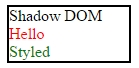
\includegraphics{kapitel2/bilder/3-shadow-dom-beispiel}
 \caption{Shadow DOM Beispiel}
 \label{fig:shadowdombeispiel}
\end{figure}

Anhand des gerenderten Outputs werden einige Dinge deutlich. Mit der Angabe des \texttt{select}-Attributs, werden im \texttt{\textless{}content\textgreater{}}-Tag nur die \texttt{\textless{}div\textgreater{}}-Tags mit der ID \texttt{hello} aus dem Shadow Root gerendert. Der Shadow Root wird dabei mittels der Anweisung \texttt{var\ root\ =\ document.querySelector('\#hello').createShadowRoot()} erzeugt. Der Paragraph mit der ID \texttt{hidden} wird hingegen nicht gerendert, da er nicht im \texttt{select} mit inbegriffen ist. Die \ac{CSS}-Regel \texttt{.content\ \{\ background-color:\ khaki;\ \}} des Eltern-\ac{HTML}-Dokuments greift nicht, da die Styles des Shadow Roots durch die Shadow Boundary gekapselt werden. Die \ac{CSS} Regel \texttt{.styled\ \{\ color:\ green;\ \}} greift allerdings, da das \texttt{\textless{}div\textgreater{}}-Element mit der Klasse \texttt{styled} aus dem Light \ac{DOM} in den Shadow \ac{DOM} projiziert wird. Außerdem können innerhalb des Templates CSS-Regeln für die beinhaltenden Elemente definiert werden, somit wird das \texttt{\textless{}div\textgreater{}}-Element ohne eine zugehörige Klasse mit der Regel \texttt{.content\ \{\ color:\ red;\ \}} auch dementsprechend in Rot gerendert.


\subsection{Browserunterstützung}\label{shadow-dom-browserunterstuetzung}

Der Shadow \ac{DOM} ist noch nicht vom \ac{W3C} standardisiert, sondern befindet sich noch im Status eines ``Working Draft'' \cite{citeulike:13879687}. Er wird deshalb bisher nur von Google Chrome ab Version 43 und Opera ab Version 33 nativ unterstützt (siehe Abbildung \ref{fig:shadowdombrowser}) \cite{citeulike:13883407}.

\begin{figure}[htbp]
 \centering
 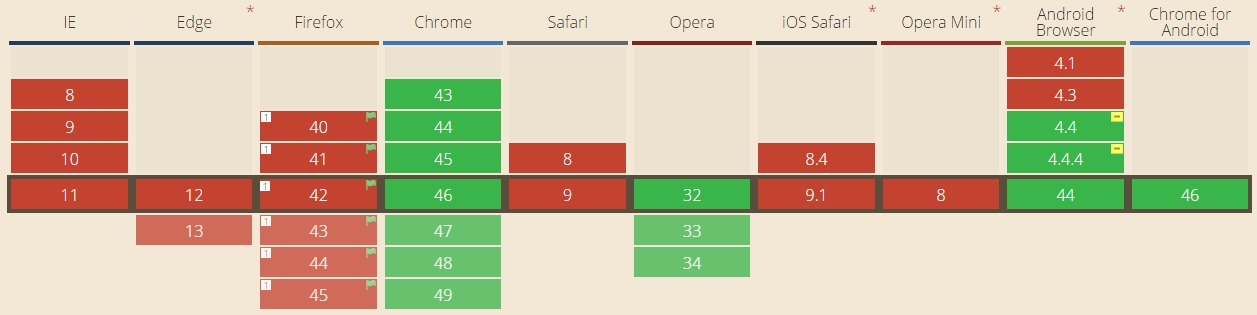
\includegraphics[width=\linewidth]{kapitel2/bilder/3-shadow-dom-browserunterstuetzung}
 \caption{Browserunterstützung des Shadow DOMs}
 \label{fig:shadowdombrowser}
\end{figure}
